\documentclass{article}
\usepackage[utf8]{inputenc}
\usepackage[margin=0.35in]{geometry}


\title{Computer Networks Lab 4}
\author{Shane Cincotta }
\date{March 30, 2020}

\usepackage{natbib}
\usepackage{graphicx}

\begin{document}

\maketitle

\begin{figure}[h!]
\centering
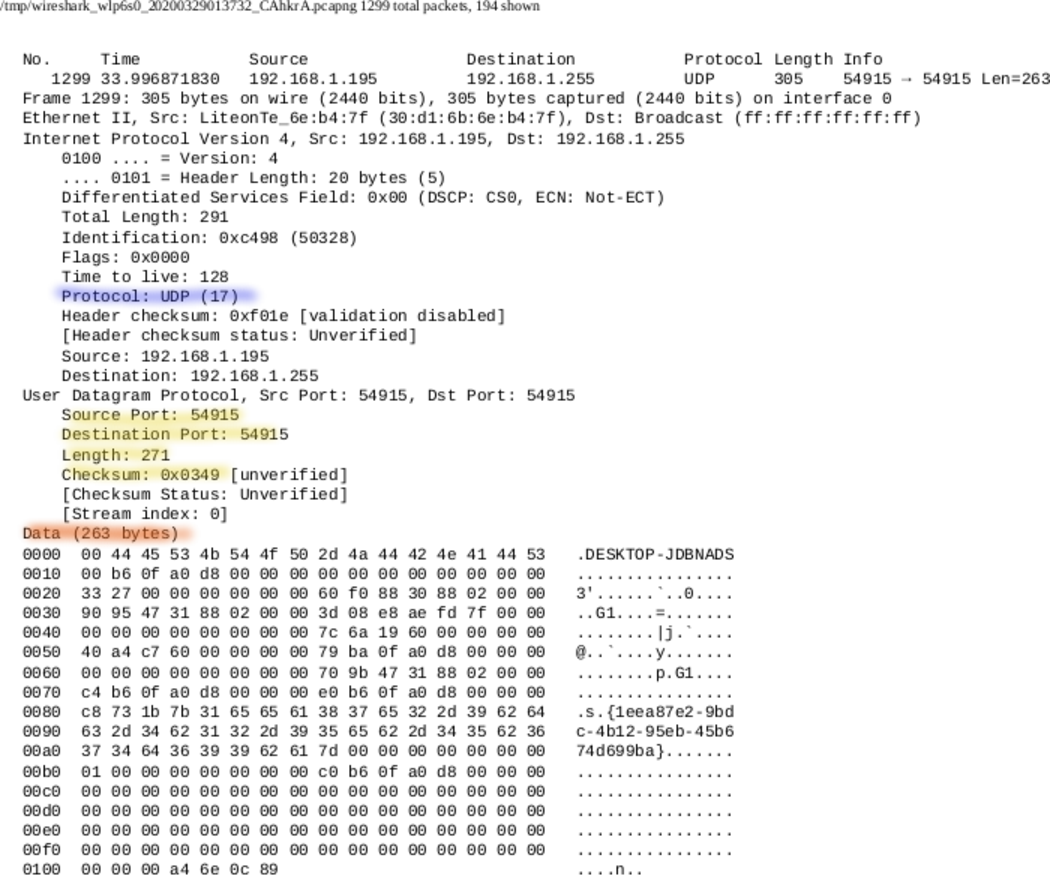
\includegraphics[scale=0.65]{Q1-7.pdf}
\caption{}
\end{figure}

\section{Select one UDP packet from your trace. From this packet, determine how many
fields there are in the UDP header. (You shouldn’t look in the textbook! Answer
these questions directly from what you observe in the packet trace.) Name these
fields}
There are four fields in the header: the source port, destination port, length and checksum.\\

\section{By consulting the displayed information in Wireshark’s packet content field for
this packet, determine the length (in bytes) of each of the UDP header fields.}
The UDP header is always  8 bytes long.  8 bytes total leaves 2 bytes per header field.\\

\section{The value in the Length field is the length of what? (You can consult the text for
this answer). Verify your claim with your captured UDP packet.}
The value of the length field is the 8 header bytes plus the data bytes.  This is verified by my packet as the length is 271, and the data is 263.  271-263 = 8 bytes left over for the header.\\

\section{What is the maximum number of bytes that can be included in a UDP payload?}
The maximum number of bytes that can be included in a UDP payload is $2^{16} - 1$ bytes minus the 8 header bytes.  This gives 65,527 bytes.\\

\section{What is the largest possible source port number?}
The largest possible port number is the largest possible 16 bit number, which is, $2^{16} - 1 = 65535$.\\

\section{What is the protocol number for UDP? Give your answer in both hexadecimal and
decimal notation. To answer this question, you’ll need to look into the Protocol
field of the IP datagram containing this UDP segment}
The protocol number for UDP is 0d17 and 0x11.\\

\section{Examine a pair of UDP packets in which your host sends the first UDP packet and
the second UDP packet is a reply to this first UDP packet. Describe the relationship between the
port numbers in the two packets.}
The relationship is that the destination port of a sent packet will be the same as the source port on the complementary packet.  Also, the source port of the reply will be the destination port of the original packet.\\

\end{document}